% http://www.idsc.ethz.ch/education/theses-semester-projects.html
% IDSC LaTeX Thesis Template
% 
% Author(s):	Eric Müller
% 				Institute for Dynamic Systems and Control
% 				Swiss Federal Institute of Technology (ETH) Zurich
% 
% Created:		2004/04/02  (Eric Mueller)
% 
% Notes: Has been tested on Windows 7 + MikTeX + TeXnicCenter
%
% Revisions: 	2009/05/29  (Soren Ebbesen)
% 				    2011/03/22	(Soren Ebbesen)
%             2013/03/08	(Soren Ebbesen)
%             2014/03/13	(Soren Ebbesen)
% ______________________________________________________________________________
\documentclass[12pt,twoside,a4paper,fleqn]{report}
\usepackage{siunitx}
\usepackage[onehalfspacing]{setspace}
%\usepackage{lineno}\linenumbers

% CHANGE HERE FOR GERMAN (german) OR MASTER THESIS (mt)!!!!!

\usepackage[english,mt]{ethidsc} % Special IDSC styles and commands      	
								 % {german}/english: language of headings, etc.
								 % {st}/bt/mt: {semester}/bachelor/master thesis


							
% Page header (don't change)____________________________________________________
\setlength{\parindent}{0em}                 % Disable parindent
\rhead[\nouppercase{\rightmark}]{\thepage}  % Special headings
\lhead[\thepage]{\nouppercase{\leftmark}}   % Special headings
\cfoot{}                                    % Special headings


% Title page (please fill in)___________________________________________________
\title{Data storage and retrieval in Ethereum DApps: cost and performance}


\studentA{Periklis Kostamis}
\ethidA{20-000-00}
\semesterA{5}
\emailA{perikost@ee.duth.gr}

%\studentB{Second Student}
%\ethidB{12-345-678}
%\semesterB{9}
%\emailB{second@student.ethz.ch}

\supervision{Prof. Dr. P.Efraimidis}
\date{March 10, 2023}

%\identification{IDSC-XX-YY-ZZ} 		% Project identifier

\infopage
\declaration

% Begin document________________________________________________________________
\begin{document}

\maketitle 							% Create title page


% Preamble______________________________________________________________________

\pagenumbering{roman} 				% Begin roman page numbering (i,ii,...)




 


%---------------------------------------------------------------------------
% Abstract

\chapter*{Abstract}
 \addcontentsline{toc}{chapter}{Abstract}
 
 The cost of interacting with a blockchain and the time required to search and retrieve information from it are important factors in the design of Decentralized Applications (DApps). The corresponding approaches for data management in Ethereum vary from pure on-chain solutions to hybrid architectures. In this work, we thoroughly examine a wide range of data management methods, including unconventional ones, and evaluate them in terms of storage cost and retrieval latency while considering the impact of recent hard forks. More precisely, we elaborate on the use of Smart Contract (SC) storage as a data store for DApps and in view of the prohibitive cost inherent to this approach, we present and compare methods for low-cost data handling in Ethereum, namely the event-logs, the transaction payload, and the almost surprising exploitation of unused function arguments. In addition, we study hybrid schemes by using IPFS and Swarm as storage platforms and Ethereum as a timestamping proof mechanism. Such schemes are especially effective when large chunks of data have to be managed. The upload and retrieval performance of these platforms and the cost associated with storing (on-chain) the identifiers of the uploaded data are of utmost importance and therefore are investigated in detail.
 
 \cleardoublepage


%---------------------------------------------------------------------------
% Acknowledgements

\chapter*{Acknowledgements}
 \addcontentsline{toc}{chapter}{Acknowledgements}

Write acknowledgements here

 \cleardoublepage

%---------------------------------------------------------------------------
% Table of contents

 \setcounter{tocdepth}{4}
 \tableofcontents

 \cleardoublepage

%---------------------------------------------------------------------------
% Symbols

\chapter*{Acronyms and Abbreviations}\label{chap:symbole}
 \addcontentsline{toc}{chapter}{Acronyms and Abbreviations}


\begin{tabbing}
 \hspace*{3.2cm}  \= \kill

write abbreviations like this\\
ET\> Evapotranspiration\\



\end{tabbing}

 \cleardoublepage

%---------------------------------------------------------------------------
 %Abstract etc.

% Chapters______________________________________________________________________

\pagestyle{fancy}               	% Fancy headings
\pagenumbering{arabic}				% Begin arabic page numbering (1,2,...)
\setlength{\parindent}{20pt}

%
\begin{table}[h]
\centering
\caption{Average performance of the five foraminifera species distribution models (SDMs) as trained on different subsets of the final choice of environmental predictors. All performance measures but the standard deviation of the partial dependency plots ($SD_{PDP}$) are calculated on the testing set. $R^2$ ranges from $-\infty$ to $+1$, with a perfect fit of the model and full variance explained indicated by a value of $+1$. Root Mean Square Error (RMSE) is an error measure, hence smaller values show higher accuracy. Nash-Sutcliffe-efficiency (NSE) indicates improvement of the model predictions over using the observation mean, with perfect model performance indicated by a value of $+1$ and a value of 0 indicating that the models perform no better than the observation mean. For a robust predictor set, the normalized standard deviation of the model predictions ($nSD$) should be as low as possible. Similarly, $SD_{PDP}$ should be low to indicate that the five SDMs learned similar PDP curves. The total rank indicates the sum of the rankings for each metric, where lower ranks show better model performance. The predictor sets are ordered by their total rank value, with our final predictor choice highlighted in bold.\\}\label{tab:model_performance_foram_predictor_sets}
\small
\begin{tabularx}{\textwidth}{lXlllllll}

\toprule
   & Predictor Set                                                              & $R^2_{test}$ & $RMSE_{test}$ & $NSE_{test}$ & $nSD_{test}$ & $SD_{PDP}$ & Total Rank \\ \midrule \midrule
   
   
1 &
  Temperature, Chlorophyll-a, MLD &
  0.13 &
  0.81 &
  0.16 &
  0.33 &
  0.19 &
  40 \\ \\
2 &
  Temperature, Chlorophyll-a, MLD, EKE, Oxygen &
  0.06 &
  0.82 &
  0.17 &
  0.34 &
  0.18 &
  46 \\ \\
3 &
  Temperature, Chlorophyll-a &
  0.09 &
  0.83 &
  0.1 &
  0.32 &
  0.18 &
  48 \\ \\
4 &
  Temperature, Chlorophyll-a, MLD, EKE &
  0.12 &
  0.81 &
  0.14 &
  0.36 &
  0.18 &
  49 \\ \\
5 &
  MLD, EKE, Salinity, Temperature, Chlorophyll-a &
  0 &
  0.84 &
  0.2 &
  0.36 &
  0.18 &
  52 \\ \\
6 &
  Temperature, Chlorophyll-a, EKE, Oxygen &
  0.09 &
  0.82 &
  0.15 &
  0.31 &
  0.22 &
  52 \\ \\
7 &
  \textbf{Temperature, Chlorophyll-a, EKE} &
  0.1 &
  0.82 &
  0.11 &
  0.33 &
  0.19 &
  53 \\ \\
8 &
  MLD, EKE, Salinity, Silicate, Temperature, Chlorophyll-a &
  -0.01 &
  0.86 &
  0.23 &
  0.41 &
  0.18 &
  63 \\ \\
9 &
  Temperature, Chlorophyll-a, MLD, Oxygen &
  0.05 &
  0.83 &
  0.17 &
  0.33 &
  0.22 &
  64 \\ \\
10 & MLD, Oxygen, EKE, Salinity, Silicate, Temperature, Chlorophyll-a & -0.09 & 0.86 & 0.22 & 0.35 & 0.21 & 71 \\ \\
11 &
  MLD, EKE, Silicate, Temperature, Chlorophyll-a &
  -0.06 &
  0.88 &
  0.2 &
  0.36 &
  0.18 &
  73 \\ \\
12 &
  Oxygen, EKE, Salinity, Temperature, Chlorophyll-a &
  0.02 &
  0.84 &
  0.19 &
  0.4 &
  0.22 &
  75 \\ \\
13 &
  Oxygen, EKE, Salinity, Silicate, Temperature, Chlorophyll-a &
  -0.02 &
  0.85 &
  0.21 &
  0.36 &
  0.23 &
  76 \\ \\
14 &
  Temperature, Chlorophyll-a, Oxygen &
  0.06 &
  0.83 &
  0.14 &
  0.32 &
  0.24 &
  77 \\ \\
15 &
  EKE, Salinity, Temperature, Chlorophyll-a &
  -0.02 &
  0.86 &
  0.18 &
  0.35 &
  0.22 &
  79 \\ \\
16 &
  MLD, Oxygen, EKE, Salinity, Temperature, Chlorophyll-a &
  -0.05 &
  0.85 &
  0.2 &
  0.36 &
  0.22 &
  80 \\ \\
17 &
  MLD, Oxygen, EKE, Silicate, Temperature, Chlorophyll-a &
  -0.06 &
  0.86 &
  0.2 &
  0.36 &
  0.21 &
  83 \\ \\
18 &
  MLD, Oxygen, Salinity, Temperature, Chlorophyll-a &
  -0.05 &
  0.85 &
  0.21 &
  0.59 &
  0.22 &
  85 \\ \\
19 &
  EKE, Salinity, Silicate, Temperature, Chlorophyll-a &
  -0.1 &
  0.89 &
  0.21 &
  0.42 &
  0.19 &
  87 \\ \\
20 &
  EKE, Silicate, Temperature, Chlorophyll-a &
  -0.09 &
  0.9 &
  0.17 &
  0.35 &
  0.2 &
  90 \\ \\
21 &
  MLD, Oxygen, Salinity, Silicate, Temperature, Chlorophyll-a &
  -0.05 &
  0.85 &
  0.25 &
  0.44 &
  0.23 &
  90 \\ \\
22 &
  Oxygen, Salinity, Temperature, Chlorophyll-a &
  0.05 &
  0.83 &
  0.18 &
  0.71 &
  0.24 &
  91 \\ \\
23 &
  MLD, Oxygen, Silicate, Temperature, Chlorophyll-a &
  -0.17 &
  0.89 &
  0.21 &
  0.41 &
  0.2 &
  96 \\ \\
24 &
  Oxygen, EKE, Silicate, Temperature, Chlorophyll-a &
  -0.04 &
  0.86 &
  0.18 &
  0.37 &
  0.22 &
  97 \\ \\
25 &
  MLD, Salinity, Silicate, Temperature, Chlorophyll-a &
  -0.17 &
  0.89 &
  0.22 &
  0.4 &
  0.22 &
  100 \\ \\
26 &
 Salinity, Silicate, Temperature, Chlorophyll-a &
  -0.14 &
  0.89 &
  0.2 &
  0.36 &
  0.22 &
  100 \\ \\
27 &
  Oxygen, Salinity, Silicate, Temperature, Chlorophyll-a &
  -0.04 &
  0.86 &
  0.2 &
  0.72 &
  0.27 &
  108 \\ \\
28 &
  MLD, Silicate, Temperature, Chlorophyll-a &
  -0.27 &
  0.93 &
  0.17 &
  0.35 &
  0.21 &
  109 \\ \\
29 &
  Silicate, Temperature, Chlorophyll-a &
  -0.27 &
  0.94 &
  0.15 &
  0.33 &
  0.22 &
  118 \\ \\
30 &
  MLD, Salinity, Temperature, Chlorophyll-a &
  -0.98 &
  1.06 &
  0.21 &
  0.37 &
  0.24 &
  122 \\ \\
31 &
  Oxygen, Silicate, Temperature, Chlorophyll-a &
  -0.17 &
  0.91 &
  0.15 &
  0.42 &
  0.21 &
  123 \\ \\
32 &
 Salinity, Temperature, Chlorophyll-a &
  -0.41 &
  0.96 &
  0.17 &
  0.41 &
  0.27 &
  143 \\ \bottomrule
\end{tabularx}
\end{table}



\chapter{Introduction}\label{chapter:introduction}

\section{Introduction}\label{sec:intro}
The Internet and World Wide Web are without a doubt two of the most significant technological achievements in human history. Since its inception, the World Wide Web has undergone a number of significant changes. It has evolved from a static network of HTML pages (Web 1.0) to an interactive ecosystem of web applications (Web 2.0), and now it's moving towards a more decentralized model (Web 3.0).

At first, websites were primarily informative. With the help of HTML, a simplistic markup language invented by the father of the World Wide Web, Tim Berners-Lee, and a home server or a cheap or even free web hosting platform, anyone could write and run their own website. As more people got involved with the web the underlying tools evolved, enabling the design of interactive websites, known as web applications. This transition marked the beginning of Web 2.0. 

In parallel, the concept of peer-to-peer networking evolved as well. Technology enthusiasts realized that by sharing their resources (bandwidth and storage capacity) they could provide the same kind of availability and throughput for their content as the huge centralized data centers of Web 2.0. Notable examples of this idea are file sharing protocols like Gnutella and BitTorent which are able to support vast networks with millions of nodes that cooperate to make content accessible. 

In January 2009, an anonymous person or group, under the pseudonym Satoshi Nakamoto published a paper that proposed a fully decentralized electronic cash system, Bitcoin \replace{[4]}{anafora. Genika kai sto ipoloipo keimeno parapanw xreiazontai anafores}, which does not rely on a central authority for the issuance of currency or the execution of transactions. The underlying technology that supports such a system is called blockchain. A blockchain network is a peer-to-peer network of nodes that follow a consensus protocol to verify and record transactions in a distributed immutable digital ledger. This technology signaled the beginning of a new era, that of Web 3.0, where interactions between users are carried out without intermediaries, in decentralized manner.

However, the true potential of the Blockchain technology was realized when Vitalik Butarin invented Ethereum in 2013. The Ethereum Blockchain is a protocol similar to Bitcoin, but its use is not limited to facilitating financial transactions. This stems from the fact that a Virtual Machine that supports a turing-complete programming language has been incorporated within its architecture. Therefore, developers can build decentralized applications that will "run" in a secure, fair and trustless setting, without relying on an intermediary. 

Similar to traditional applications, decentralized applications consist of code and a set of data which, depending on the case, significantly varies in size. However, storing data in Ethereum is associated with a monetary cost. For a limited volume of data this cost is reasonable, otherwise it's prohibitive, thus limiting the use of Ethereum as a storage medium for applications. To address this weakness, part of the Ethereum team proceeded with the design of Swarm, a distributed storage system capable of hosting large data sets at a lower cost. Apart from Swarm, there are other distributed storage systems such as IPFS, Sia, Storj, and decentralized databases like \comment{BigChainDB}{einai deprecated pleon opote den xerw an prepei na to anaferoume} and OrbitDB that can be coupled with Ethereum to facilitate fully decentralized applications. 

Combining blockchain technology, particularly Ethereum, with other decentralized peer-to-peer storage solutions will significantly contribute to the process of \hl{redefining/transforming} the World Wide Web into what Tim Berners-Lee originally envisioned: a decentralized open platform with no single point of failure, where users have full control of their data. 

\section{Motivation \& Contributions}\label{sec:}
While the number of individuals that use blockchain systems is growing \comment{significantly}{We need a citation that prove it}, concerns about the performance and cost of using public blockchains like Ethereum \citep{buterin_2014} discourage widespread adoption. In particular, storing data in Ethereum is expensive. However, Decentralized Applications (DApps) running on top of the blockchain, usually manage some of their data on-chain. The \comment{narrow range}{What did you mean?} of design patterns for fully Decentralized Applications \citep{wohrer_2021} and the lack of comprehensive research about on-chain data handling, hinders the development of efficient Smart Contracts (SCs) and leads to higher costs that are laid onto the users of DApps. Minimizing the use of SC storage in favor of more cost-efficient alternatives or using distributed file systems such as IPFS \citep{benet_2014} and Swarm \citep{tron_2020} alongside Ethereum, could ameliorate this problem \comment{.}{kaneis anafora tis texnologies alla oxi to provlima, tha psaxw kamia anafora na valoume}


According to this information, we define our research question: how can data be efficiently managed in Ethereum DApps?
In our attempt to answer this, we examine a wide range of storage options in Ethereum as well as a hybrid on-chain/off-chain architecture and make a comparative study to explore the advantages and disadvantages of each approach. 

% TODO: propose the use of an alternative data store in Ethereum
{\bf Main contributions.} In this work, we:
\begin{itemize}[topsep=0pt, itemsep=0pt]
\item{Propose the use of the alternative data stores in Ethereum.}
\item{Cost-wise compare all available data stores.}
\item{Examine the time needed to retrieve data from the Ethereum blockchain.}
\item{Evaluate hybrid approaches utilizing IPFS and Swarm.}
\add{\item Creation of a network of IPFS/Swarm nodes in Grid5000 for the evaluation of the hybrid approach in a real network.}
\end{itemize}

More specifically, we make a detailed (cost-wise) analysis \comment{regarding the cost}{mhpws mesa se komma h na to diatipwsoume diaforetika} of the available on-chain data management methods. Firstly, we evaluate the most straightforward approach, that is, storing data directly in SC storage. Since SC storage is not immutable like the corresponding data structures where transactions and receipts are recorded, we also consider the cost of updating and deleting contract data. 

Then we exploit EVM’s logging functionality to store data in transaction receipts. Similarly, we examine the transaction's data field as an alternative data store and also propose an extension to this approach, which we term as \emph{``Unused Function Parameters''}. All these methods are evaluated in terms of gas consumption. By doing so, we are able to demonstrate that indeed there are other data structures within Ethereum’s architecture that can be used as a form of cheaper data stores.

% All these methods are evaluated in terms of gas consumption and the associated implementation complexity is discussed. By doing so, we are able to demonstrate that indeed there are other data structures within Ethereum’s architecture that can be used as a form of cheaper data stores, but also inform the reader...

In order to provide an up-to-date \hl{overview/perspective} of the storage methods we examine, we monitored all upgrades of Ethereum that occurred in parallel to our study and re-executed our experiments whenever deemed necessary. As a result, we outline the impact that some Ethereum Improvement Proposals (EIPs) had on gas consumption. Specifically, we discuss the EIPs that were enforced after the Muir Glacier fork and introduced modifications related to the gas metering and refund mechanisms. Comments on the latter provide valuable insight on the cost of deleting data and complement the discussion on data handling in SC storage.

Furthermore, we evaluate the retrieval performance of Ethereum for each of the aforementioned data stores. Aiming to be thorough, we also take into account the fact that recently retrieved data is cached by the operating system. Regarding the event-logs, additional remarks on the role that Bloom filters (BF) have in the data retrieval process, are made.

The last contribution of this work is an assessment of on-chain/off-chain hybrid schemes. In this context, we examine the cost linked to storing (on-chain) identifiers of data hosted in IPFS or Swarm. Obviously, all of Ethereum's data stores can be used for this purpose. We present only the use of the SC storage and the event-logs, but one can use the discussion in section \ref{sec:evaluation_ethereum} as a guide and draw conclusions about the efficiency of the rest of the methods. In addition, we review the upload and download performances of IPFS and Swarm which must be considered in conjunction with the performance of Ethereum in order get an overall perspective of such a scheme. 

\section{Thesis Structure}\label{sec:organization}
% The structure of this paper is as follows. In Section 2 we discuss the related work. In the next Section, we compare the available data handling practices for on-chain data and describe the main differences between IPFS and Swarm, from a theoretical point of view. In Section 4 we define the criteria of our experiments, outline the environment in which they were conducted and discuss our results both in terms of cost and performance. In the last Section, we gather our conclusions. 

\cleardoublepage
\chapter{Methods}\label{chapter:methods}
\section{Experiment}\label{sec:experiment}
\subsection{Experimental setup}\label{subsection:set-up}
\section{Data processing}\label{sec:experiment}



\cleardoublepage
\chapter{Results}\label{chapter:results}


\cleardoublepage
\chapter{Discussion}\label{chapter:discussion}


\cleardoublepage
\chapter{Conclusion and Outlook}\label{chapter:Conclusion}

\cleardoublepage

% ...

% Appendix______________________________________________________________________
\appendix
\chapter{Appendix}\label{chapter:appendix}

\begin{table}[H]
\centering
\begin{small}
\caption{Accumulated measurements for experiment \textit{simple} in IPFS. The dataset consists of 1050 samples in total (including failures), with retrieval failure ratio of $\sim 4\%$ }
\label{tab:normal}
\begin{tabular}{@{}lccccccc@{}}
\toprule
Size & Mean & Median & IQR & Skewness & Min & Max & Sample Size \\ \midrule
4KB & 472.96 & 211.66 & 109.01 & 3.69 & 30.04 & 5408.44 & 140\\
16KB & 135.24 & 150.64 & 28.92 & -1.06 & 30.90 & 203.29 & 143\\
64KB & 176.44 & 175.63 & 90.05 & -0.19 & 34.75 & 382.46 & 143\\
256KB & 247.11 & 239.92 & 161.51 & 1.17 & 38.85 & 712.93 & 145\\
1MB & 514.83 & 234.93 & 202.04 & 11.63 & 52.27 & 27258.04 & 146\\
4MB & 635.02 & 431.22 & 246.71 & 2.64 & 103.36 & 3260.39 & 145\\
16MB & 1797.22 & 1306.89 & 688.50 & 2.70 & 338.36 & 9525.16 & 144\\
\bottomrule
\end{tabular}
\end{small}
\end{table}


\begin{table}[H]
\centering
\caption{Accumulated measurements for each experiment in Swarm without outliers.}
\resizebox{\textwidth}{!}{%
\begin{tabular}{@{}lcccccccc@{}}
\toprule
Experiment    & \multicolumn{7}{c}{Data Size}          & Failures (\%) \\ \midrule
& 4kb  & 16kb  & 64kb  & 256kb  & 1mb  & 4mb  & 16mb              \\ \midrule
normal & 35.91 & 207.6 & 302.56 & 475.75 & 1126.42 & 3727.21 & 9815.11 & 9 \\
no-cache  & 50.49 & 258.35 & 314.25 & 467.14 & 1206.17 & 3418.18 & 8391.32 & 9 \\
disconnect  & 52.21 & 179.63 & 344.74 & 467.44 & 1247.89 & 3507.51 & 8713.88 & 7 \\
no-cache-disconnect  & 51.54 & 152.27 & 327.29 & 441.47 & 1208.57 & 3497.87 & 8567 & 10 \\
\bottomrule
\end{tabular}
}
\end{table}


\begin{table}[H]
\centering
\begin{small}
\caption{Accumulated measurements for each experiment in IPFS without outliers.}
\begin{tabular}{@{}lcccccccc@{}}
\toprule
Experiment    & \multicolumn{7}{c}{Data Size}          & Failures (\%) \\ \midrule
& 4kb  & 16kb  & 64kb  & 256kb  & 1mb  & 4mb  & 16mb              \\ \midrule
normal & 199.88 & 154.76 & 171.33 & 194.54 & 212.07 & 402.53 & 1209.93 & 4 \\
no-cache  & 160.85 & 51.96 & 72.66 & 97.88 & 116.75 & 195.59 & 638.54 & 24 \\
disconnect  & 135.36 & 124.72 & 1168.58 & 310.82 & 1360.46 & 469.56 & 1275.26 & 37 \\
no-cache-disconnect  & 151.11 & 163.59 & 263.22 & 313.85 & 1758.96 & 759.66 & 1801.96  & 53 \\
\bottomrule
\end{tabular}
\end{small}
\end{table}



\begin{table}[H]
\centering
\begin{small}
\caption{Accumulated measurements for IPFS without outliers.}
\begin{tabular}{@{}lccccccc@{}}
\toprule
Size & Mean & Median & Skewness & Min & Max & Sample Size & Outliers \\ \midrule
4KB & 146.85 & 145.64 & 0.31 & 6.99 & 394.83 & 326 & 89\\
16KB & 113.8 & 141.63 & -0.32 & 3.13 & 243.88 & 328 & 62\\
64KB & 153.98 & 158.9 & 0.67 & 3.32 & 655.62 & 295 & 89\\
256KB & 210.55 & 174.56 & 1.4 & 38.86 & 891.33 & 318 & 82\\
1MB & 737.98 & 310.51 & 1.49 & 9.67 & 3600.76 & 391 & 19\\
4MB & 564.25 & 415.7 & 1.82 & 99.65 & 2399.45 & 363 & 49\\
16MB & 1359.79 & 1216.78 & 1.21 & 297.5 & 4592.43 & 369 & 29\\
\bottomrule
\end{tabular}
\end{small}
\end{table}

\begin{table}[H]
\centering
\begin{small}
\caption{Accumulated measurements for Swarm without outliers.}
\begin{tabular}{@{}lccccccc@{}}
\toprule
Size & Mean & Median & Skewness & Min & Max & Sample Size & Outliers \\ \midrule
4KB & 43.66 & 50.49 & 0.74 & 1.19 & 182.76 & 356 & 39\\
16KB & 218.75 & 196.73 & 0.58 & 2.66 & 662.08 & 389 & 6\\
64KB & 330.4 & 319.61 & 0 & 3.32 & 677.07 & 380 & 15\\
256KB & 483.43 & 465.3 & 0.04 & 4.69 & 978.37 & 381 & 14\\
1MB & 1276.7 & 1217.82 & 0.65 & 675.32 & 2259.57 & 378 & 22\\
4MB & 3623.02 & 3520.14 & 0.5 & 2165.56 & 5889.15 & 387 & 17\\
16MB & 9037.03 & 8914.55 & 0.46 & 5822.69 & 14261.94 & 159 & 10\\
\bottomrule
\end{tabular}
\end{small}
\end{table}






\begin{table}[H]
\centering
\begin{small}
\caption{Accumulated measurements for each experiment in IPFS without outliers (degroot-miletus-nancy).}
\begin{tabular}{@{}lcccccccc@{}}
\toprule
Experiment    & \multicolumn{7}{c}{Data Size}          & Failures (\%) \\ \midrule
& 4kb  & 16kb  & 64kb  & 256kb  & 1mb  & 4mb  & 16mb              \\ \midrule
normal & 188.38 & 149.39 & 158.54 & 167.08 & 292.41 & 461.01 & 1816.65 & 0 \\
no-cache  & 146.06 & 141.99 & 143.93 & 152.68 & 261.62 & 524.04 & 1955.46 & 3 \\
disconnect  & 189.47 & 306.23 & 1252.18 & 1281.77 & 1751.59 & 1458.82 & 3536.62 & 12 \\
no-cache-disconnect  & 198.14 & 170.18 & 1230.74 & 372.82 & 1961.7 & 2011.86 & 3162.53 & 27 \\
\bottomrule
\end{tabular}
\end{small}
\end{table}


\begin{table}[H]
\centering
\begin{small}
\caption{Accumulated measurements for experiment \textit{disconnect} in IPFS. The dataset consists of 665 samples in total (including failures), with retrieval failure ratio of $\sim 6.5\%$ }
\label{tab:disconnect}
\begin{tabular}{@{}lccccccc@{}}
\toprule
Size & Mean & Median & IQR & Skewness & Min & Max & Sample Size \\ \midrule
4KB & 899.4 & 144.2 & 1040.53 & 2.14 & 6.99 & 8551.52 & 141\\
16KB & 1234.05 & 139.67 & 1051.18 & 5.94 & 3.13 & 29803.37 & 128\\
64KB & 2417.38 & 1264.5 & 2557.39 & 3.92 & 3.32 & 29352.31 & 123\\
256KB & 1474.87 & 335.85 & 1385.74 & 6.63 & 42.83 & 30001.96 & 130\\
1MB & 1431.46 & 1360.46 & 2015.44 & 0.83 & 9.67 & 5071.64 & 136\\
4MB & 1783.34 & 494.24 & 1737.18 & 5.14 & 99.65 & 27082.3 & 139\\
16MB & 2184.65 & 1363.14 & 2050.4 & 5.38 & 297.5 & 26714.33 & 133\\
\bottomrule
\end{tabular}
\end{small}
\end{table}













\begin{table}[H]
\centering
\begin{small}
\caption{IPFS: accumulated measurements for our machine (degroot). The dataset consists of 665 samples in total (including failures), with retrieval failure ratio of $\sim 6.5\%$ }
\label{tab:degroot_ipfs}
\begin{tabular}{@{}lcccccc@{}}
\toprule
Size & Mean & Median & Skewness & Min & Max & Sample Size \\ \midrule
4KB & 1421.16 & 242.18 & 1.18 & 139.82 & 5819.67 & 88\\
16KB & 1065.02 & 170.23 & 2.54 & 128.68 & 10072.69 & 86\\
64KB & 1308.95 & 249.04 & 3.58 & 131.93 & 14766.25 & 87\\
256KB & 981.47 & 313.59 & 1.89 & 143.75 & 5293.09 & 90\\
1MB & 1249.65 & 385.42 & 1.22 & 195.49 & 5071.64 & 89\\
4MB & 1799.89 & 516.34 & 4.38 & 337.33 & 21345.4 & 93\\
16MB & 2476.33 & 1499.17 & 1.72 & 995.34 & 9461.04 & 89\\
\bottomrule
\end{tabular}
\end{small}
\end{table}

\begin{table}[H]
\centering
\begin{small}
\caption{IPFS: accumulated measurements for Lille site. The dataset consists of 665 samples in total (including failures), with retrieval failure ratio of $\sim 44\%$ }
\begin{tabular}{@{}lcccccc@{}}
\toprule
Size & Mean & Median & Skewness & Min & Max & Sample Size \\ \midrule
4KB & 556.61 & 130.76 & 5.58 & 33.68 & 10806.75 & 56\\
16KB & 199.35 & 123.73 & 4.32 & 28.48 & 2182.87 & 51\\
64KB & 485.99 & 175.87 & 2.23 & 40.17 & 3269.44 & 52\\
256KB & 491.22 & 201.17 & 2.25 & 49.33 & 3402.34 & 52\\
1MB & 1325.06 & 272.27 & 6.46 & 58.97 & 27258.05 & 55\\
4MB & 1298.11 & 464.68 & 6.03 & 108.31 & 22407.71 & 54\\
16MB & 1618.79 & 1098.98 & 2.91 & 304.16 & 9793.04 & 52\\
\bottomrule
\end{tabular}
\end{small}
\end{table}





\begin{table}[H]
\centering
\begin{small}
\caption{Swarm: accumulated measurements for our machine (degroot). The dataset consists of 458 samples in total (including failures), with retrieval failure ratio of $\sim 9\%$ }
\begin{tabular}{@{}lcccccc@{}}
\toprule
Size & Mean & Median & Skewness & Min & Max & Sample Size \\ \midrule
4KB & 125.64 & 106.78 & 1.13 & 1.19 & 375.95 & 65\\
16KB & 355.39 & 356.69 & 0.35 & 6.21 & 731.93 & 65\\
64KB & 506.36 & 455.06 & 0.8 & 6.14 & 1034.46 & 65\\
256KB & 701.1 & 659.04 & 0.52 & 10.05 & 1484.6 & 65\\
1MB & 1752.64 & 1718.43 & -0.5 & 16.36 & 2673.54 & 65\\
4MB & 4703.53 & 4606.77 & -1.05 & 39.54 & 7884.58 & 66\\
16MB & 12671.97 & 11706.08 & 0.8 & 8623.28 & 18851.85 & 25\\
\bottomrule
\end{tabular}
\end{small}
\end{table}

\begin{table}[H]
\centering
\begin{small}
\caption{Swarm: accumulated measurements for Lille site. The dataset consists of 474 samples in total (including failures), with retrieval failure ratio of $\sim 8\%$ }
\begin{tabular}{@{}lcccccc@{}}
\toprule
Size & Mean & Median & Skewness & Min & Max & Sample Size \\ \midrule
4KB & 31.59 & 31.63 & 4.54 & 2.41 & 398.32 & 67\\
16KB & 129.7 & 62.44 & 1.51 & 3.38 & 515.84 & 67\\
64KB & 262.84 & 267.23 & 0.09 & 3.72 & 588.63 & 67\\
256KB & 384.88 & 365.31 & 0.45 & 5.01 & 811.72 & 67\\
1MB & 991.81 & 976.45 & -0.61 & 10.82 & 1796.9 & 68\\
4MB & 2874.76 & 2855.04 & -1.46 & 34.05 & 4680.03 & 68\\
16MB & 8463.23 & 8544.81 & -0.14 & 5822.69 & 10991.23 & 30\\
\bottomrule
\end{tabular}
\end{small}
\end{table}



\begin{figure}[htbp]
\centerline{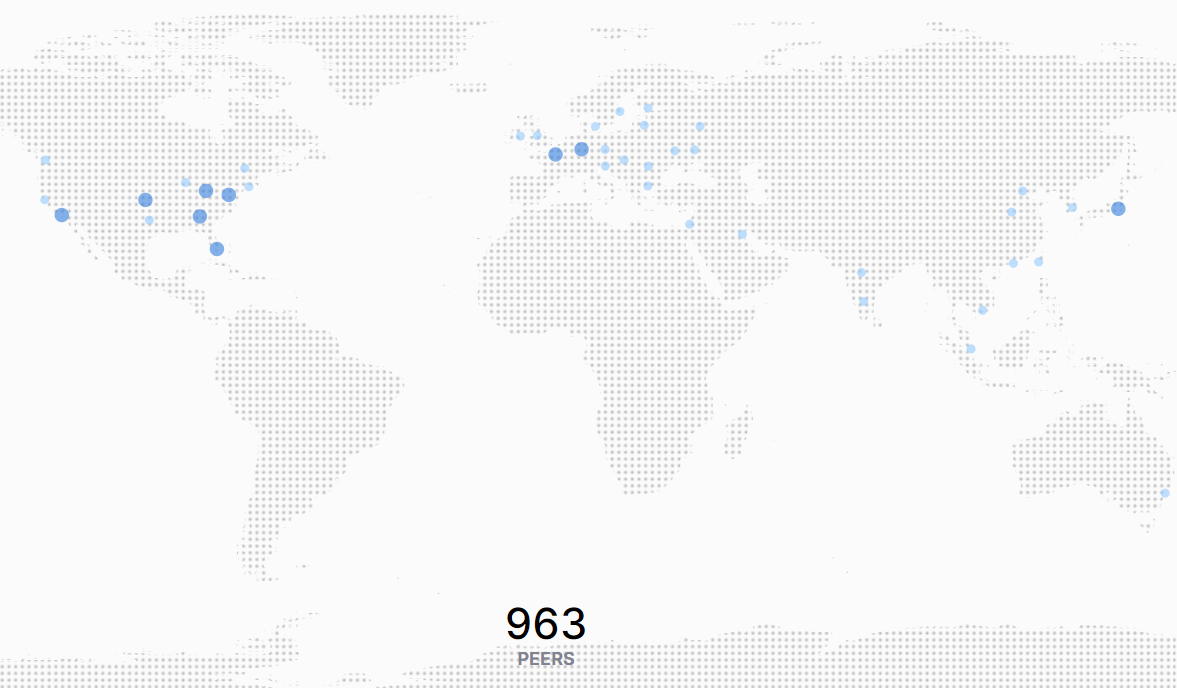
\includegraphics[width=\textwidth]{figs/ipfs_peers.png}}
\caption{EIP standardization process.}
\label{fig:ipfs_peers}
\end{figure}


% Bibliography__________________________________________________________________
% Literature (Additional references can be added to the .bib-file manually, or by using, for example, the free application JabRef). Compile in the following order: latex -bibtex -latex -latex

%\bibliographystyle{plain}
\begin{footnotesize}
\bibliographystyle{apalike}
\bibliography{references}
\end{footnotesize}

\end{document}
